\documentclass[manuscript]{aastex}

\usepackage{float}

\begin{document}

\title{Positional Abudance Trends in Red Clump Star in the Milky Way}
\author{Natalie Price-Jones}

\section{Background}
The question of galaxy formation is a relatively open one. Although simulations have succeeded in tracing the broad strokes of formation history, there are subtle connections that remain unexplored. Observational evidence implies empirical relations between properties of different bulk sections of galaxies, like bulge and disk velocity dispersion, as well as correlations between large and small scales, such as the $M_{\rm BH}-\sigma$ relation. Some of these observations also serve as indirect evidence for dark matter, but the influence of this elusive substance on a galaxy's dynamical properties is not fully understood. Understanding a galaxy's formation history offers an opportunity to investigate the source of these relations. This may allow for predictions about how galaxies will continue to evolve and interact.

In distant galaxies, we may study a galaxy's bulk properties, but our position in the Milky Way offers us the opportunity to examine individual stars in detail. These individual elements at small scales are influenced by bulk properties, the dynamical evolution of the galaxy. By searching for correlations in properties including effective temperature, gravitational acceleration and elemental abundances we can learn about where and how populations of stars form and what happens to them over their lifetimes. 

Finding this information relies on stellar surveys that extend far beyond the solar neighbourhood. Large-volume spectroscopic survey data from the APO Galactic Evolution Experiment (APOGEE), the Large Sky Area Multi-Object Fibre Spectroscopic Telescope (LAMOST) and upcoming data from the Gaia mission will offer rich and detailed information about hundreds of thousands of stars. Even with data reduction pipelines in place, interpreting that data to find meaningful results will be challenging. However, these results might offer constraints on theories of the Milky Way's formation and evolution, which in turn hints at similar processes at work in other galaxies.  


\section{Research Plan}

\subsection{Data}
This work will focus analysing the spectra of a sample of red clump stars from APOGEE's Data Release 12. These stars are selected according to cuts in gravity, effective temperature, and metallicity, and leave us with a sample of 19936 stars. These stars trace, to some extent, the stellar population of the Milky Way. Time spent in the red clump is short compared to the lifetime of a star, so the sample is biased towards locating younger stars. Data on these stars comes in the form of infrared (H-band) spectra covering a wavelength range from 1.514 $\mu$m to 1.696 $\mu$m (with some small nm gaps between detectors). APOGEE's DR12 pipeline provides data on abundances of 15 elements (C, N, O, Na, Mg, Al, Si, S, K, Ca, Ti, V, Mn, Fe, Ni) as well as effective temperature ($T_{\rm eff}$), surface gravity ($\log(g)$) and alpha-element enhancements ([$\alpha$/Fe]).

\begin{figure}[H]
\centering
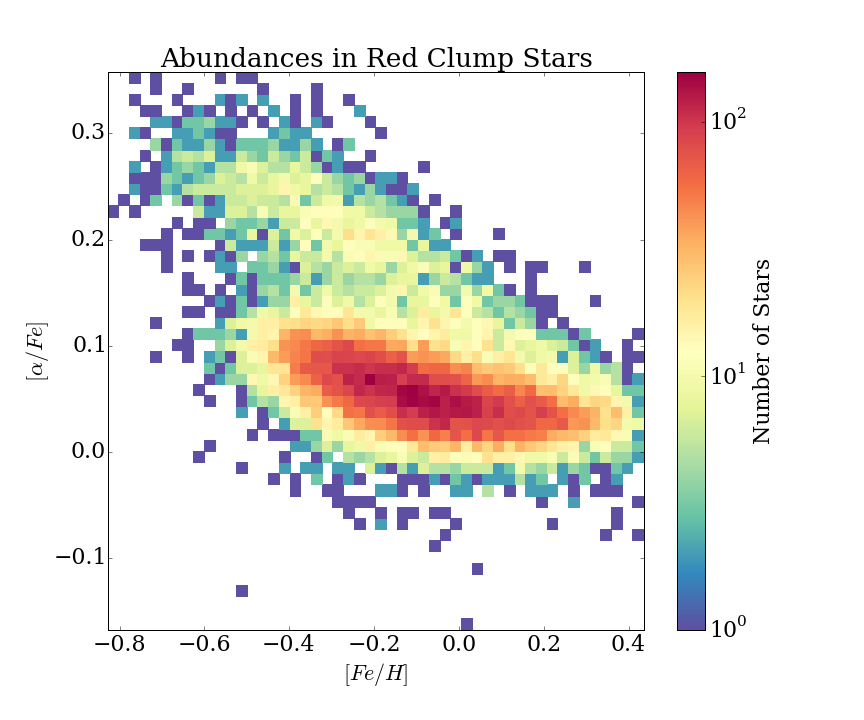
\includegraphics[width = \linewidth]{alpha_vs_fe.png}
\caption{$\alpha$-enhancement vs iron abundance for 19936 red clump stars from APOGEE Data Release 12.}
\label{fig:abun}
\end{figure}

\end{document}